%!TEX root = ../../report.tex

\subsubsection{Noise} % (fold)
\label{ssub:noise}


``To generate irregular procedural textures, we need an irregular primitive function, usually called noise" \cite{Ebert2002}. It's a pseudorandom function that gave the goal to break the monotony of a pattern and make it look more random.
Perlin Noise is the most known and used noise function. It was created by Ken Perlin, for the movie Tron 1982 with the aiming to generate natural looking textures.
The psedorandom property is important and a true random function like \emph{white noise} would not do the job. If we generate a texture based on white noise, we would like that it 
With this pseudorandom function, it's generated a sequence of values that are interpolated to generate a coherent noise. With the composition of several layers of this noise it's build a texture that look natural and with fractal like structure.


\begin{figure}[htbp]
	\centering
	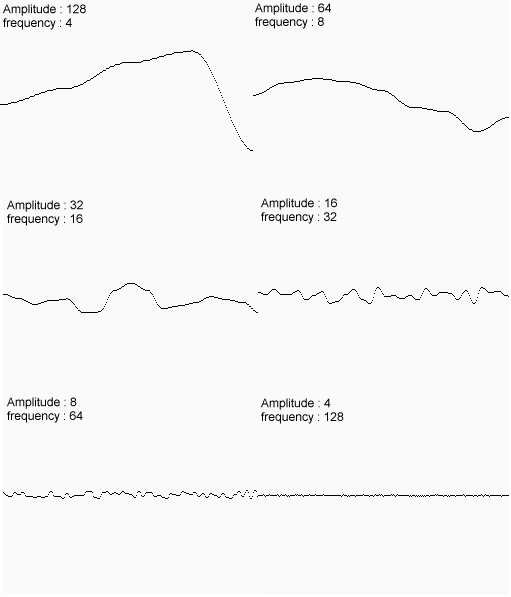
\includegraphics[width=0.75\textwidth]{img/Theory/Perlin_Noise/Merge.png}
	\caption{Different noise functions}
	\label{fig:merge}
\end{figure}



For instance, the Figure~\ref{fig:merge} shows the result of six noise functions with different frequencies and amplitudes. And the sum of all this functions is the exibithed in the Figure~\ref{fig:noise} \cite{NoisesELIAS}.



\begin{figure}[htbp]
	\centering
	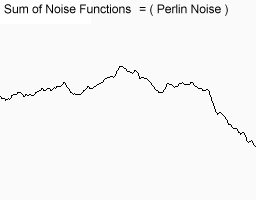
\includegraphics[width=0.65\textwidth]{img/Theory/Perlin_Noise/perlin1.png}
	\caption{``You may even imagine that it looks a little like a mountain range."}
	\label{fig:noise}
\end{figure}




% subsubsection noise (end)
